\documentclass[a4paper]{article}

%% Language and font encodings
\usepackage[english]{babel}
\usepackage[utf8x]{inputenc}
\usepackage[T1]{fontenc}

%% Sets page size and margins
\usepackage[a4paper,top=3cm,bottom=2cm,left=3cm,right=3cm,marginparwidth=1.75cm]{geometry}

%% Useful packages
\usepackage{amsmath}
\usepackage{graphicx}
\usepackage[colorinlistoftodos]{todonotes}
\usepackage[colorlinks=true, allcolors=blue]{hyperref}

\title{Autoignition time}
\author{Artur Kuriata}

\begin{document}
\maketitle


\section{Introduction}

This section will be dedicated to simulation of autoignition time of ethane. Using Cantera program to analize influence of pressure and concentration of water in the mixture on autoignition time.

\section{Mathematical model}
The mixture of ethane and water is located in ideal reactor with total mol mass of : Nitrogen - 3.76 mol , Oxygen - 1 mol , ethane -1 mol and water with 0 - 1.44 mol. In first part reactor temperature is changed from 1176 K to 1538 K and the changes of temperature  in function  of distance where measured.In second part pressure is changed from 0,8 bar to 1 bar and the changes of pressure in function where measured. In the third part we add water to methane with 0 - 20 percent and the the changes of water percentage in mixture in function is measured.

\section{Program description}
	\subsection{Basic part of program}
   \textbf{Importing libraries}
   
   import sys
   
import numpy as np

from cantera import *

import cantera as ct

from pylab import *

import csv

\textbf{Creating gas object used to evaluate all thermodynamic, kinetic, and transport
properties.}

gas = Solution('gri30.cti')

\textbf{Specifying the number of time steps,the time step size and borders of each parameter}

nt = 100000

dt = 1.e-6  

Tmin = 0.65

Tmax = 0.85

npoints = 11

pmin= 0.8

pmax = 1

wmin=0

wmax=1.44

$Autoignition_cas = np.zeros(npoints, 'd')$

$FinalTemp_cas = np.zeros(npoints, 'd')$

$mfrac_cas = np.zeros([npoints, gas.n_species], 'd')$

\textbf{Looping over the three variables}

for l in range(npoints):

\hspace{5,35mm}$w[l]= wmin + (wmax +wmin) * l / (npoints - 1)$
   
\hspace{5,35mm}$procent = (w[l]/(5.76+w[l]))*100$
   
\hspace{10,70mm}for k in range(npoints):
    
\hspace{10,70mm}$pi[k]= pmin +(pmax-pmin) * k / (npoints-1)$
        
\hspace{10,70mm}$one_atm= one_atm *pi[k]$
        
\hspace{10,70mm}for j in range(npoints):
        
\hspace{16,05mm}$Ti2[j] = Tmin + (Tmax - Tmin) * j / (npoints - 1)$

\hspace{16,05mm}$Ti[j] = 1000 / Ti2[j]$
            
\hspace{16,05mm} \textbf{Set gas state, always at stoichiometry} 
        
\hspace{16,05mm}$gas.TPX = Ti[j], one_atm, ('C2H6:1,O2:1,N2:3.76,H2O:'+str(w[l]))$
            
\hspace{16,05mm}\textbf {Create the ideal batch reactor}
       
\hspace{16,05mm}$r = ct.IdealGasReactor(gas)$
            
\hspace{16,05mm}\textbf{ create a reactor network consisting of the single batch reactor}
       
\hspace{16,05mm}$ sim = ct.ReactorNet([r])$
           
\hspace{16,05mm}\textbf{Initial simulation time}
   
\hspace{16,05mm}$time = 0.0$
            
\hspace{16,05mm}\textbf{Loop for nt time steps of dt seconds.}
    
\hspace{16,05mm}for n in range(nt):
            
\hspace{21,40mm}$time += dt$
                
\hspace{21,40mm}$sim.advance(time)$
                
\hspace{21,40mm}$tim[n] = time$
                
\hspace{21,40mm}$temp_cas[n] = r.T$
                
\hspace{21,40mm}$mfrac_cas[j][:] = r.thermo.Y$

\textbf{Getting time of autoignition}

\hspace{16,05mm}$Dtmax = [0, 0.0]$

\hspace{16,05mm}for n in range(nt - 1):

\hspace{21,40mm}$dtemp_cas[n] = (temp_cas[n + 1] - temp_cas[n]) / dt$
 
\hspace{21,40mm}$if (dtemp_cas[n] > Dtmax[1]):$

\hspace{26,75mm}$Dtmax[0] = n$

\hspace{26,75mm}$Dtmax[1] = dtemp_cas[n]$
\textbf{Printing the result of calculation}

\hspace{16,05mm}Autoignition     = ((tim[Dtmax[0]] + tim[Dtmax[0] + 1]) / 2.)

\hspace{16,05mm}print ('For ' + str(Ti[j]) +',p='+str(pi[k])+',st='+str(w[l])+ ', Autoignition time =

\hspace{16,05mm}(s) ' + str(Autoignition))

\hspace{16,05mm}$Autoignition_cas[j] = Autoignition * 1000  $

\hspace{16,05mm}$FinalTemp_cas[j] = temp_cas[nt - 1]$

\textbf{Making plot of the results of calculations}

\hspace{10,70mm}$plot(Ti2, Autoignition_cas, '^', color='orange')$

\hspace{10,70mm}$xlabel(r'Temp [1000/K]', fontsize=20)$

\hspace{10,70mm}$ylabel("Autoignition [ms]")$

\hspace{10,70mm}$title(r'Autoignition of C_{2}H_{6} + Air mixture at Phi = 1, P ='+ str(pi[k]) +'bar and H_{2}O-'$

\hspace{10,70mm}$+str(procent)+'of mixture', fontsize=22,horizontalalignment='center')$

\hspace{10,70mm}$axis([0.60, 0.90, 0.0, 100.0])$

\hspace{10,70mm}$grid()$

\hspace{10,70mm}$show()$

\section{Results}
Program returns plot returns time of autoignition of mixture of ethane and water of mixture temperature in the reactor.

\begin{figure}

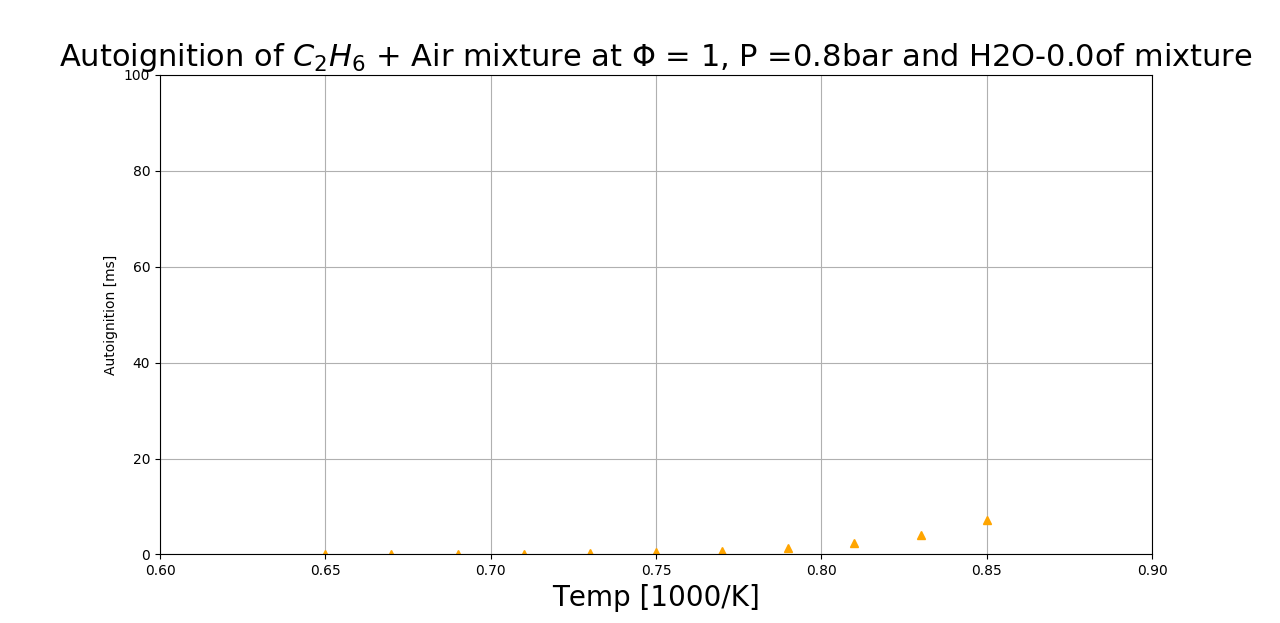
\includegraphics[width=1\textwidth]{przyk_ad.png}
\caption{\label{fig:1}Autoignition time of an ethane mixture with water in function of reactor temperature.}
\end{figure}



\section{Conclusion}
Results from calculations for different pressures and concentration of water estabilished division indicates that increasing these parameters extend time of mixture autoignition.






\end{document}